%\subsection{Only NQM as a Loss}
\label{experiments:01.1:Only_NQM}
Therefore, as a first attempt at the use of the NQM for robustness, we simply defined the NQM itself as a loss:

\begin{align}
    \mathrm{NQM}\ :=\ \frac{\sum_{s\in SD} (s)} {\sum_{m\in\mu}}, \qquad
    SD = \sqrt{\frac{\sum^N_{i=1}(v_i-\mu)^2}  {N}}, \qquad
    \mu = \frac{\sum^N_{i=1}v_i}  {N}  
\end{align}

However, using this as a loss function does not work because the values below the square root in the SD and the denominator of the NQM can become zero and are then undefined.
To avoid zero-squarerooting, we choose to add an $\varepsilon$ of $e^{-8}$. To avoid zero-division, we choose to add a smoothing value of $1$. This makes the NQM loss:

\begin{align}
    \mathrm{NQM}\ :=\ \frac{\sum_{s\in SD} (s) {\color{red}+1}} {\sum_{m\in\mu} {\color{red}+1}}, \qquad
    SD = \sqrt{\frac{\sum^N_{i=1}(v_i-\mu)^2}  {N} {\color{red} + \varepsilon}}, \qquad
    \mu = \frac{\sum^N_{i=1}v_i}  {N}  
\end{align}


Loss function technically works. The model can be trained on it, but it will simply label the entire image within very few epochs since the NQM will be zero if the denominator becomes as large as possible, which is the case if the prediction is maximized. So, a model trained on this loss function will not predict anything because it will predict everything.\\
The loss function is usually a function of a model output and a label $\ell(y_i, f_\theta(x_i))$. However, since the NQM is only a function of the model output $\ell(f_\theta(x_i))$, it is not possible that a model trained on the NQM can predict anything. Therefore, it is a crude but sensible first step in exploration.


\begin{figure}[h!]
    \centering
    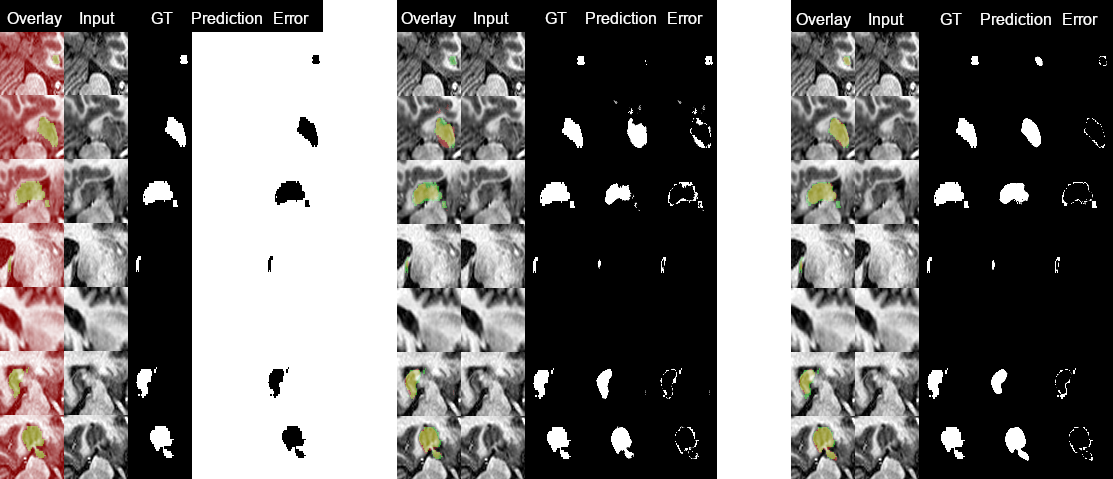
\includegraphics[width=\linewidth]{Graphics/Experiments/4.1.1_DiceBce_GT_vs._NQM_only_v2.png}
    \caption{Example image volumes (input) with ground truth labels (GT), predictions and errors. The overlay shows the input image with false positive (red), true positive (yellow), false negative (green). The model on the left was trained on the NQM as loss and clearly predicts nothing at all by simply labeling everything (overlay all red, label all white). The output stays this way from epoch 2 on. For comparison, the middle and right models were trained on DiceBCE. The middle one shows the output after 10 epochs, the right one after 500 epochs.}
    \label{fig:exp.01.1:DiceBce_vs_NQM_only}
\end{figure}